%%%%%%%%%%%%%%%%%%%%%%%%%%%%%%%%%%%%%%%%%%%%%%%%%%%%%%%%%%%%%%%%%%%%%%%%%%%%%%%%
%%%%%%%%%%%%%%%%%%%%%%%%%%%%%%%%%%%%%%%%%%%%%%%%%%%%%%%%%%%%%%%%%%%%%%%%%%%%%%%%
%%                                                                            %%
%% opintnaytepohja.tex versio 3.20 (2018/08/31)                               %%
%% Opinnäytepohja käytettäväksi aaltothesis.sty (versio 3.20) -tyylitiedoston %%
%% kanssa.                                                                    %%
%% Toimiakseen paketti tarvitsee pdfx.sty v. 1.5.84 (2017/05/18) tai uudempi. %%
%% The LaTeX template file to be used with the aaltothesis.sty (version 3.20) %%
%% style file.                                                                %%
%% This package requires pdfx.sty v. 1.5.84 (2017/05/18) or newer.            %%
%%                                                                            %%
%% This is licensed under the terms of the MIT license below.                 %%
%%                                                                            %%
%% Written by Luis R.J. Costa.                                                %%
%% Currently developed at the Learning Services of Aalto University School of %%
%% Electrical Engineering by Luis R.J. Costa since May 2017.                  %%
%%                                                                            %%
%% Copyright 2017-2018, by Luis R.J. Costa, luis.costa@aalto.fi,              %%
%% Copyright 2017-2018 Swedish translations in aaltothesis.cls by Elisabeth   %%
%% Nyberg, elisabeth.nyberg@aalto.fi and Henrik Wallén,                       %%
%% henrik.wallen@aalto.fi.                                                    %%
%% Copyright 2017-2018 Finnish documentation in the template opinnatepohja.tex%%
%% by Perttu Puska, perttu.puska@aalto.fi, and Luis R.J. Costa.               %%
%% Copyright 2018 English template thesistemplate.tex by Luis R.J. Costa.     %%
%% Copyright 2018 Swedish template kandidatarbetsbotten.tex by Henrik Wallen. %%
%%                                                                            %%
%% Permission is hereby granted, free of charge, to any person obtaining a    %%
%% copy of this software and associated documentation files (the "Software"), %%
%% to deal in the Software without restriction, including without limitation  %%
%% the rights to use, copy, modify, merge, publish, distribute, sublicense,   %%
%% and/or sell copies of the Software, and to permit persons to whom the      %%
%% Software is furnished to do so, subject to the following conditions:       %%
%% The above copyright notice and this permission notice shall be included in %%
%% all copies or substantial portions of the Software.                        %%
%% THE SOFTWARE IS PROVIDED "AS IS", WITHOUT WARRANTY OF ANY KIND, EXPRESS OR %%
%% IMPLIED, INCLUDING BUT NOT LIMITED TO THE WARRANTIES OF MERCHANTABILITY,   %%
%% FITNESS FOR A PARTICULAR PURPOSE AND NONINFRINGEMENT. IN NO EVENT SHALL    %%
%% THE AUTHORS OR COPYRIGHT HOLDERS BE LIABLE FOR ANY CLAIM, DAMAGES OR OTHER %%
%% LIABILITY, WHETHER IN AN ACTION OF CONTRACT, TORT OR OTHERWISE, ARISING    %%
%% FROM, OUT OF OR IN CONNECTION WITH THE SOFTWARE OR THE USE OR OTHER        %%
%% DEALINGS IN THE SOFTWARE.                                                  %%
%%                                                                            %%
%%                                                                            %%
%%%%%%%%%%%%%%%%%%%%%%%%%%%%%%%%%%%%%%%%%%%%%%%%%%%%%%%%%%%%%%%%%%%%%%%%%%%%%%%%

\documentclass[finnish, 12pt, a4paper, elec, utf8, a-1b, online]{aaltothesis}
%\documentclass[finnish, 12pt, a4paper, elec, utf8, a-1b]{aaltothesis}

\usepackage{graphicx}

\usepackage{amsfonts, amssymb, amsbsy, amsmath}

\usepackage{longtable, multirow, booktabs}

% Rotation: \rot[<angle>][<width>]{<stuff>}
\newcommand{\rot}[3]{\makebox[#1][c]{\rotatebox{#2}{#3}}}

% Vertical: \vertical[<angle>][<width>]{<stuff>}
\newcommand{\vertical}[1]{\rot{12pt}{90}{#1}}

\usepackage{biblatex}

\addbibresource{refs.bib}

\degreeprogram{Automaatio- ja informaatioteknologia}

\major{Informaatioteknologia}

\code{ELEC3015}

\univdegree{BSc}

\thesisauthor{Aapo Kiiso}

\thesistitle{Web-sivuston ulkoasun personointi}

\place{Espoo}

\date{xx.xx.2022}

\supervisor{Titteli Samuli Aalto}

\advisor{TkT Markku Laine}

\uselogo{aaltoBlue}{''}

\keywords{avainsana 1\spc{}avainsana 2\spc{}}

\thesisabstract{
}

\copyrighttext{Copyright \noexpand\copyright\ \number\year\ \ThesisAuthor}
{Copyright \copyright{} \number\year{} \ThesisAuthor}

\begin{document}

\makecoverpage{}

\makecopyrightpage{}

\begin{abstractpage}[finnish]
\end{abstractpage}

\thesistableofcontents{}

\mysection{Käsitteet ja lyhenteet}

\subsection*{Käsitteet}

\begin{tabular}{ll}
    mukauttaminen & kohdentaminen käyttäjälle tai käyttäjäryhmälle sopivaksi \\
    personointi   & kerättyyn tietoon perustuva automaattinen mukauttaminen  \\
    kustomointi   & valintoihin ja asetuksiin perustuva mukauttaminen
\end{tabular}

\subsection*{Lyhenteet}

\begin{tabular}{ll}
    CSS  & Cascading Style Sheets    \\
    HTML & HyperText Markup Language \\
    RWD  & Responsive Web Design
\end{tabular}

\cleardoublepage{}

\section{Johdanto}

Ihmisen ja tietokoneen välinen vuorovaikutus on ollut tietojenkäsittelytieteessä
tutkimuksen kohteena henkilökohtaisen tietokoneen läpimurrosta 1970- ja
1980-lukujen vaihteesta lähtien~\cite{10.1145/800178.810088}. Yksi tutkimuksen
tavoitteista on ollut löytää menetelmiä mukauttaa tietokoneen ohjelmistoja
kullekin käyttäjälle sopivaksi.

Ohjelmistojen mukauttaminen voidaan jakaa karkeasti kahteen osa-alueeseen.
Ensinnäkin kustomoinnilla (engl.~\textit{customization}) tarkoitetaan käyttäjän
itse tekemää mukauttamista. Toisekseen personoinnilla
(engl.~\textit{personalization}) tarkoitetaan automaattista mukauttamista
käyttäjästä kerätyn tiedon perusteella.~\cite{10.1108/03090560710737534}

Aikaisessa tutkimuksessa tutkittiin nimenomaan ohjelmistojen mukauttamista
kustomoinnin avulla, eli muun muassa tarjoamalla käyttäjälle asetuksia
tarpeettomien toimintojen piilottamiseen. Ajan kuluessa tutkimuksen painopiste
on siirtynyt kustomoinnista personoinnin puolelle~\cite{viite?}.

Alkuaikoina ohjelmistojen jakelu levykkeiden ja muiden fyysisten
tiedontallennusvälineiden muodossa hankaloitti personointiin liittyvän
teknologian tutkimusta ja kehitystä, sillä ohjelmistopäivitysten jakelu
käyttäjille oli hidasta ja kallista. 1990-luvulla yleistyneitä internet- eli
web-sivustoja (engl.~\textit{website}) ei tarvitse perinteisten ohjelmistojen
tapaan jaella käyttäjille, vaan palvelimelta voidaan tarjoilla aina uusin versio
web-sivustosta. Internetin mahdollistama palveluntarjoajan ja loppukäyttäjän
välinen reaaliaikainen vuorovaikutus johti myös osaltaan personointia
hyödyntävän liiketoiminnan, kuten sähköisen kaupankäynnin ja sosiaalisen median
kehittymiseen. Internetin käytön leviäminen arkielämään 1990- ja 2000-lukujen
kuluessa kiihdytti personointiin kohdistuvaa tutkimusta ja kehitystä
edelleen~\cite{10.1108/03090560710737534}.

Vaikka web-sivustojen personointia on tutkittu verrattain pitkään, käytännön
hyödyntäminen toimialalla on vielä harvinaista~\cite{viite?}.
Web-sivuston ulkoasu suunnitellaan nykyäänkin lähtökohtaisesti ihmisen toimesta,
ja myös ulkoasusuunnitelman tulkitseminen ja ohjelmoiminen lopulliseksi
web-sivustoksi on manuaalista työtä. Käyttäjille tai edes käyttäjäryhmille ei
siis ole kustannustehokasta suunnitella personoituja versioita sivustoista.
Yhden ja saman version jakelu kaikille web-sivuston käyttäjille ei ole
kuitenkaan aina optimaalista, sillä käyttäjillä on usein eri tarpeita muun
muassa kulttuuritaustasta ja iästä riippuen~\cite{viite?}.

Työn tarkoitus on selvittää mitä menetelmiä web-sivuston ulkoasun eri osien
personointiin on olemassa. Tarkasteltavia osia ovat muun muassa web-sivuston
asettelu, kirjasin- ja värivalinnat sekä valikot. Työ tarkastelee myös eri
personointimenetelmien toimintatapoja. Monet tarkasteltavista menetelmistä
perustuvat matemaattisen optimointiin, mutta hyödyntävät myös
käyttöliittymäsuunnittelun heuristiikkoja kuten tekstin luettavuuskriiterejä
tuloksissaan. Oma lukunsa ovat koneoppimiseen perustuvat menetelmät, joiden
opetusdatana on käytetty esimerkiksi olemassa olevia web-sivustoja. Työ myös
vertailee menetelmien käyttöönoton kustannuksia saavutettaviin hyötyihin, ja
pyrkii tätä kautta löytämään matalan kynnyksen persononointimenetelmät, joista
saa suurimman hyödyn.

\clearpage

\section{Tausta}

Web-kehitys on muuhun ohjelmistokehitykseen verrattuna nuori ala ja
edelleen jatkuvassa murroksessa. Tässä kappaleessa esitellään web-kehityksen
nykytilannetta työn taustatiedoksi.

\subsection{Web-suunnittelu}

Web-suunnittelu (engl.~\textit{web design}) on käytännön tasolla lähellä muita
graafisen suunnittelun aloja kuten printtisuunnittelua, vaikka mediana web
tarjoaa paljon enemmän mahdollisuuksia vuorovaikutukseen. Web-suunnittelun
päätuotos eli arkikielessä \textit{leiska} (engl.~\textit{layout}) on
ei-vuorovaikutteinen vektorikuva siitä, miltä toteutettavan web-sivuston tulee
näyttää. Leiskan lisäksi suunnittelija tuottaa usein rajoitetun interaktiivisia
prototyyppejä, joilla sivuston toimintaa voi esitellä leiskan kautta esimerkiksi
asiakkaalle ennen toteutusta. Leiskaan tehdään tarvittavat mukautukset eri
käyttäjäryhmille vain ennalta sovittujen määrittelyjen ja palvelumuotoilun
(engl.~\textit{service design}) pohjalta. Yleisin tällainen mukautus on omien
leiskojen tuottaminen eri laitetyypeille, kuten mobiili-, tabletti- ja
työpöytälaitteille. Laitetyyppeihin perustuvaa mukauttamista kutsutaan
responsiiviseksi web-suunnitteluksi (engl.~\textit{responsive web design}),
josta kerrotaan lisää luvussa~\ref{responsive-web-design}. Varsinaista
personointia leiskoihin ei yleensä sisällytetä.

\subsection{Moderni web-kehitys}

Web-kehittäjän (engl.~\textit{web developer}) tehtävä on kääntää leiska
toimivaksi web-sivustoksi. Ei-vuorovaikutteisesta luonteestaan huolimatta leiska
ei nykyään ole enää pelkkä rasterikuva (engl.~\textit{raster image}), toisin
kuin yleisesti vielä 2000-luvun alussa. Vektorimuotoiseen leiskaan on upotettu
kaikki web-kehittäjän tarvitsemat yksityiskohdat ulkoasun toteuttamiseen, kuten
kirjasintyyppi ja -koko, marginaalit ja värikoodit. Web-kehittäjä hyödyntää
leiskan käsittelyyn joko samoja työkaluja kuin suunnittelija, tai varta vasten
leiskojen käsittelyyn tarkoitettuja kehittäjätyökaluja.

Karkeasti yleistäen web-kehityksessä on pääosassa kolme teknologiaa: HTML, CSS
ja JavaScript. HTML-merkintäkielen avulla määritetään web-sivuston rakenne ja
eri osien rakenteellinen merkitys. Web-selain (engl.~\textit{web browser})
ymmärtää rakenteen eri osien merkityksen ja pystyy piirtämään ne sivulle
oikealla tavalla. CSS-säännöstön avulla määritetään web-sivuston osien tyyli ja
asettelu, eli se on HTML-merkintäkielen lisäksi merkittävässä osassa leiskaa
toteuttaessa. JavaScript on ainoa web-alustalla kattavasti tuettu varsinainen
ohjelmointikieli. Sillä on mahdollista luoda vuorovaikutusta käyttäjän ja
sivuston välille.

Nykyään web-kehittäjä rakentaa sivustoja harvemmin enää pelkästään näillä
kolmella perusteknologialla, vaan niiden päälle on kehitetty teknologioita ja
kirjastoja jotka vähentävät toistuvaa työtä ja huolehtivat jossain määrin
hyvistä käytänteistä kuten saavutettavuudesta. Nämä teknologiat hyödyntävät
enenevissä määrin JavaScript-ohjelmointikieltä, mikä on tuonut web-kehitystä
lähemmäs perinteisempää ohjelmistokehitystä. Aiemmin web-sivustoja oli yleistä
rakentaa lähes ilman ohjelmointityötä pelkän HTML-merkintäkielen ja
CSS-tyylisäännöstön avulla. Sivustojen käytettävyyttä parannettiin kevyen
JavaScript-skriptauksen kera siellä ja täällä, mutta varsinainen ohjelmointityö
rajoittui yleensä palvelinpuolelle. Palvelinpuolen kehitystä ei tässä työssä
esitellä tai käsitellä työn rajauksesta johtuen.

Sittemmin tärkeä edistysaskel web-kehityksessä on tapahtunut 2010-luvun
loppupuolen jälkeen, kun JavaScript-käyttöliittymäkirjastot ovat yleistyneet
merkittävästi. Yleisimmät käyttöliittymäkirjastot vuonna 2022 ovat React ja Vue.
Käyttöliittymäkirjastot abstraktoivat perinteisen web-kehityksen kuten
HTML-rakenteen luomisen, CSS-tyylittelyn ja JavaScript-toiminnallisuuden
rakentamisen semanttisten web-komponenttien sisälle. Komponentit enkapsuloivat
jonkin tietyn toiminnallisuuden, ja niitä on suhteellisen helppo
uudelleenkäyttää myöhemmin. Komponentit myös mahdollistavat osaltaan
suunnittelujärjestelmien (engl.~\textit{design system}) luomisen jo projektin
alussa. Suunnittelujärjestelmä sisältää yleensä projektin komponenttikirjaston,
joka käsittää sivuston rakennuspalikat kuten painikkeet, otsikot ja lomakkeet.

Tähän vielä selkeytystä komponenteista ja mitä muuta fronttikirjastot tekee.
Selkeytystä myös design system osalta. Jotain muuta ehkä myös, esimerkiksi valmiit
komponenttikirjastot tai frameworkit (Bootstrap, Tailwind, jne)?

\subsection{Ulkoasun tuottaminen koneellisesti}

Tähän ulkoasun generoinnista asiaa. Nimenomaan ei-personoinnin näkökulmasta,
vaan yleisiä menetelmiä

\clearpage

\section{Personointi}

Personointi osana ihmisen ja tietokoneen välistä vuorovaikutusta on laaja aihe,
ja työ on tarkoituksella rajattu vain web-sivuston ulkoasun personointiin
näkökulman tarkentamiseksi. Työ keskittyy pääasiassa ulkoasun personointiin
vaikka myös web-sivuston sisällön personointia sivutaan, sillä sisällön
personointi on aiheena laaja ja kasvattaisi työn rajausta liian suureksi.
Sisällön personointiin kuuluu esimerkiksi sosiaalisen median alustojen
suosittelualgoritmit ja web-mainonnan kohdennus, jotka eroavat menetelmiltään
merkittävästi web-sivuston ulkoasun personoinnista. Ulkoasun personointiin
kuuluu kuitenkin olennaisena osana käyttäjälle tärkeän sisällön korostaminen,
jota tarkastellaan luvussa~\ref{layout-personalization}.

\subsection{Hyödyt ja haitat}

Personoinnilla tarkoitetaan käyttäjästä kerätyn tiedon perusteella tehtävää
automaattista mukauttamista. Kerätty tieto voi olla hyvin erilaisista lähteistä,
kuten asiointihistoriasta, julkishallinnon rekistereistä tai web-sivuston
tapauksessa käyttäytymisestä sivustolla. Tieto jonka pohjalta personointia
tehdään voi olla myös käyttäjän itse ilmoittamaa, joskin tällöin puhutaan
yleensä kustomoinnista. Personointia voidaan tehdä missä tahansa rajapinnassa
jossa on käyttäjän ja palvelun välistä vuorovaikutusta, kuten toimipiste-,
puhelin- tai web-asioinnissa. Tämä työ keskittyy web-asioinnin personointiin
ja nimenomaan web-sivuston ulkoasun personointiin.

Tarve personoinnille vaihtelee web-sivuston mukaan, mutta yleisesti voidaan
todeta että personoinnin tavoitteena on ohjata käyttäjän toimintaa web-sivuston
palveluntarjoajan tavoitteiden mukaisesti, ja yleensä nimenomaan joko lisätä
palveluntarjoajan tuloja tai vähentää sen menoja. Esimerkiksi tyypillisen
verkossa toimivan uutismedian tavoite on kerätä tuloja näyttämällä mainoksia
artikkelien yhteydessä. Personoimalla käyttäjälle näytettäviä sisältöjä
esimerkiksi korostamalla tälle mielenkiintoisia aiheita, käyttäjä saadaan
lukemaan enemmän artikkeleja ja täten kasvatettua uutismedian mainostuloja. Sitä
vastoin esimerkiksi kunta voisi pyrkiä vähentämään asiointiin liittyviä soittoja
puhelinneuvontaan, jonka ylläpitäminen on kallista. Sivuston etusivua
personoimalla kunta voisi nostaa juuri käyttäjälle ajankohtaiset lomakkeet heti
sivun alkuun, ja täten helpottaa käyttäjän asiointia.

Personoinnilla voidaan siis säästää rahaa, mutta sen kautta on mahdollista saada
myös yleishyödyllisempiä hyötyjä. Web-sivuston personointi mahdollistaa
yksilöllisen tiedonvälityksen kokoluokassa, joka ei aiemmin ole ollut
mahdollista. Printtimedia skaalautuu kyllä hyvin ja sen kautta tietoa on ollut
mahdollista levittää laajalle jo vuosisatoja, mutta sen personointi on liki
mahdotonta tai ainakin erittäin kallista. Toinen ääripää eli tiedonvälitys
henkilöltä toiselle on aina personoitua, mutta se ei skaalaudu. Julkinen valta
ja muut yleishyödylliset toimijat voivat siis hyödyntää personointia
tiedonvälityksessä tavoittaakseen suurempia yleisöjä. Tästä on ollut hyötyä
esimerkiksi COVID-19 -pandemian aikana, kun rokotekampanjoita on voitu kohdentaa
verkossa tärkeille yleisöille~\cite{viite?}.

Tähän vielä personoinnin hyödyistä saavutettavuuden näkökulmasta ja mukautuminen
eri fyysisiin ympäristöihin (esim isompi fontti auringonpaisteessa).

Personoinnissa on kuitenkin myös selkeitä kipukohtia. Personointi perustuu
käyttäjästä kerättyyn tietoon. Tietoa kerätään mahdollisesti monesta eri
kanavasta, ja on tärkeää että tietojen keräämiseen on aina käyttäjän suostumus.
Tietolähteiden lisääntyessä käyttäjä ei välttämättä enää ole kartalla siitä,
mitä tietoa on suostunut luovuttamaan ja mihin. Tietojen luovutuspyyntöihin myös
turtuu nopeasti, mistä esimerkkinä on EUn GDPR-direktiivin myötä yleistyneet
evästesuostumuslomakkeet. Suostumusta kysytään lähes jokaisella
web-sivustolla, koska web-analytiikka ja kohdennettu mainonta on niin
yleistä. Asenteet sisällön personoinnin osalta ovat muuttuneet kielteisempään
suuntaan, kun vielä 90-luvulla sisällön personointi nähtiin verkkoon siirtyvän
printtimedian pelastajana~\cite{adams_1995}.

Arkielämän teknistyessä käyttäjälle ei myöskään ole välttämättä aina selvää,
mitä kaikkea tietoa on edes mahdollista kerätä. Tietoja kuten hiiren liike,
näppäimistösyöte, laitetiedot ja jossain määrin myös selailuhistoria ovat
web-sivuston käytettävissä. Laitetietojen pohjalta sivusto voi muodostaa
käyttäjästä sormenjäljen, jota on käytännössä mahdoton muuttaa tai pyyhkiä pois
vaihtamatta laitetta. Evästeiden avulla isot mainosverkostot pystyvät seuraamaan
käyttäjää sivustolta toiselle ja personoimaan mainontaa selailukäyttäytymisen
perusteella.

Personointi ei aina ole edes haluttua. Monet alustapohjaiset teknologiayritykset
ovat viime vuosina panostaneet erilaisiin suosittelualgoritmeihin kohdentaakseen
sisältöään paremmin. Suosittelualgoritmit toimivat hyvin suurelle osalle
käyttäjäkunnasta, mutta saattavat hankaloittaa palvelun käyttöä pienelle osalle,
johon kuuluvat eivät istu hyvin algoritmin luokittelijaan. Suosittelualgoritmit
ovat myös korvanneet palveluiden aiemmin käyttäjälle tarjoamia
kustomointimahdollisuuksia kuten sisällön järjestelyasetuksia, mikä on
hankaloittanut palvelun käyttöä~\cite{patel_2022}.

Jo aiemmin mainittu COVID-19 rokotetietoisuuden kohdentaminen on myös
kaksiteräinen miekka. Jos hyväntahtoiset toimijat kuten terveysvirastot pystyvät
personoimaan tiedonvälitystä avainryhmille, sama onnistuu myös pahantahtoisilta
toimijoilta. Välittämällä kyseenalaista tietoa kuten salaliittoteorioita
vastaanottavaisille ryhmille voidaan lyödä kiilaa yhteiskunnan sisälle.

Tämän työn aihe eli web-sivuston ulkoasun personointi on kuitenkin verrattain
harmiton personoinnin osa-alue. Sen haittapuolena on lähinnä lisääntynyt
tekninen monimutkaisuus käytetystä menetelmästä riippuen. Saavutetut hyödyt ovat
web-sivuston palveluntarjoajan lisääntyvässä asiakastyytyväisyydessä ja sitä
kautta lisääntyvissä tuloissa tai vähentyvissä menoissa.

\subsection{Näkökulmat ulkoasun personointiin}\label{personalization-aspects}

Tässä työssä personointia tarkastellaan eri näkökulmista. Näkökulmat jakaantuvat
karkeasti kahteen ryhmään, käyttäjälähtöisiin näkökulmiin ja ympäristölähtöisiin
näkökulmiin.

Osa käyttäjälähtöisistä näkökulmista perustuu käyttäjän fyysisiin
ominaisuuksiin. Käyttäjällä voi olla esimerkiksi rajoitteita, kuten näkö- ja
liikuntarajoitteita, jotka vaikuttavat merkittävästi web-sivuston käyttöön.
Muita fyysisiä ominaisuuksia, jotka vaikuttavat web-sivuston käyttöön, ovat ikä
ja sukupuoli. Fyysisten ominaisuuksien lisäksi myös kulttuuritausta ja kieli,
koulutustaso, kiinnostuksen kohteet, sosiaaliset verkostot ja jopa mieliala ovat
ominaisuuksia, joiden perusteella web-sivustoa voidaan personoida käyttäjälle.
Lisäksi myös web-sivuston aiempi käyttöhistoria voi vaikuttaa personointiin.

Ympäristölähtöiset näkökulmat liittyvät web-sivuston selailuun käytettävän
laitteen ominaisuuksiin ja toisaalta myös laajemmin käyttöympäristön
ominaisuuksiin. Laitteen ominaisuuksia, joiden perusteella personointia voidaan
tehdä, ovat laitteen näyttökoko ja suorituskyky. Laajemmin käyttöympäristöön
liittyviä personoitavia näkökulmia ovat verkkoyhteyden nopeus, sijainti sekä
vuoden- ja kellonaika. Laitteen antureita voidaan hyödyntää lähiympäristön
havainnoimiseen, jolloin personoinnissa voidaan hyödyntää ympäristön kirkautta,
lämpötilaa, taustamelun äänenvoimakkuutta sekä liike-ominaisuuksia, kuten
tärinää ja nopeutta.

\subsection{Asettelun personointi}\label{layout-personalization}

Sivun asettelu määrittää web-sivuston perusrakenteen ja sivun sisällön
keskinäisen järjestyksen. Tyypillisesti web-sivuston yksittäisellä sivulla on
vähintään ylätunniste (engl.~\textit{header}), sisältöalue
(engl.~\textit{content area}) ja alatunniste (engl.~\textit{footer}).
Ylätunniste ja alatunniste pysyvät yleensä suurin piirtein muuttumattomina
sivustolla navigoidessa, mutta sisältöalueen sisältö luonnollisesti vaihtuu
sivun mukaan. Ylätunniste ja alatunniste ovat valikonomaisia sivuston osia.
Ylätunniste sijaitsee aina sivun alussa ja alatunniste sivun lopussa. Niiden
asettelun personointi ei ole mielekästä, joten niitä ei tarkastella enempää
tässä luvussa.

Valikoiden asettelua on toki myös mahdollista personoida. Valikoiden asettelu
eroaa normaalista sisällöstä hivenen siksi, että valikon vaihtoehdoilla on
vähemmän vapausasteita verrattuna sisällön asetteluun. Vaihtoehtojen järjestys
voi muuttua, niitä voidaan piilottaa ja niitä voidaan korostaa esimerkiksi
lihavoinnilla. Ne eivät siis esimerkiksi voi lähtökohtaisesti siirtyä valikon
ulkopuolelle. Valikoiden personointi onkin siis ulkoasullisesti triviaalia, ja
menee enemmän sisällön personoinnin puolelle.

Sisältöalueen asettelu perustuu nykyään lähtökohtaisesti ruudukkorakenteeseen
(engl.~\textit{grid layout}). Ruudukko koostuu sivustosta ja päätelaitteen
näyttökoosta riippuen yleensä n.~1--16 sarakkeesta (engl.~\textit{column}),
jotka on erotettu toisistaan vakiosuuruisella marginaalilla
(engl.~\textit{margin}). Sarakkeiden leveys, joka on kääntäen verrannollinen
sarakkeiden määrään, perustuu suhteelliseen osaan saatavilla olevasta
ruudukkoalueen (engl.~\textit{grid container}) leveydestä, ja sarakkeiden leveys
muuttuu yhdessä ruudukkoalueen kanssa. Ruudukkoalueelle sijoittuvat elementit
(engl.~\textit{element}), kuten tekstipalstat ja kuvat, voivat kattaa yhden tai
useamman sarakkeen leveyden. Elementtien leveys määritetään kuitenkin nimenomaan
sarakkeiden kautta, eivätkä ne voi vapaasti laajentua leveyssuunnassa niiden
sisällön kasvaessa. Sen sijaan elementit laajenevat tarvittaessa
pituussuunnassa. Tyypillisesti web-sivustot eivät mahdukaan kokonaan kerralla
näytölle, vaan niitä pitää vierittää alaspäin jolloin lisää sisältöä tulee
näkyville.

\subsubsection{Responsiivinen web-suunnittelu}\label{responsive-web-design}

Ennen 2010-lukua asettelu tehtiin lähtökohtaisesti staattisesti, tarkoittaen
että sivun sisältöalueella oli ennalta määrätty leveys. Leveys oli yleensä
maksimissaan 1024 pikseliä, joka oli senaikaiset päätelaitteet huomioon ottaen sopiva
koko~\cite{viite?}. Sisältöalueen leveys ei muuttunut päätelaitteen mukaan. Sivun suunnittelu
ja toteutus oli verrattain helppoa, koska hankalista asettelun rajatapauksista
ei tarvinnut huolehtia. Toisaalta staattisesti rakennetut sivustot alkoivat olla
hankalia käyttää älypuhelinten yleistyessä, sillä sivustojen käyttö pienellä
näyttökoolla vaati zoomausta sisällön erottamiseksi.

Nykypäivänä on tyypillistä, että sivuston asettelu mukautuu päätelaitteen
näyttökokoon. Näyttökokoon perustuvaa asettelun mukautumista kutsutaan
responsiiviseksi web-suunnitteluksi (engl.~\textit{responsive web design}),
joskin termi kattaa myös muita mukauttamisperusteita, kuten paperille
tulostuksen. Sivuston perustuessa ruudukkorakenteeseen asettelu mukautuu
automaattisesti näyttökoon muutoksiin, sillä sarakkeiden leveys on määritetty
suhteessa ruudukkoalueeseen. Asettelua voi kuitenkin parantaa entisestään
lisäämällä sarakkeiden määrää näyttökoon kasvaessa, ja vähentämällä sarakkeiden
määrää näyttökoon pienentyessä. Tällä tavalla esimerkiksi työpöytälaiteella
vierekkäin näkyvät elementit voidaan mobiililaitteella asetella allekkain,
jolloin ne ovat pienelläkin näyttökoolla yhtä suuria kuin työpöytälaiteella.

Asettelun muuttaminen näyttökoon muuttuessa tapahtuu leveyteen perustuvien
pysäytyspisteiden (engl.~\textit{breakpoint}) avulla. Pysäytyspisteet
määritetään \textit{media queries} -tekniikan~\cite{Rivoal:12:MQ} avulla, joka
mahdollistaa muun muassa CSS-tyylien kohdentamisen päätelaitteen ominaisuuksien
mukaan. Pysäytyspisteisiin pohjautuva asettelun mukauttaminen on yleinen ja
helppo tapa mukauttaa sivuston asettelua eri päätelaitteille. Pysäytyspisteiden
avulla asettelu mukautetaan yleensä vähintään niin, että puhelimille,
tableteille ja työpöytälaitteille on kullekin oma asettelunsa.

\subsubsection{Suunnittelijan työkalut}

Personointimenetelmät voivat toimia suunnittelijan työkalujen kontekstissa.
Tällöin ne on helpompi ottaa käyttöön, koska työkalut on lähtökohtaisesti samat
kaikilla ja niihin integroituminen voidaan toteuttaa lisäosa-tyyppisten
ratkaisujen kautta. Nykyään suosittuja web-suunnitteluun käytettäviä
ohjelmistoja ovat muun muassa Sketch, Figma ja Adobe XD, joihin kaikkiin on
mahdollista rakentaa lisäosia. Perinteisempiä työkaluja edustavat Adoben
tuoteperheen Photoshop ja Illustrator, joiden käyttö web-suunnittelussa on
vähentynyt merkittävästi.

Yksi suunnittelijoille suunnattu apukeino on Pang et al.~\cite{Pang2016}
esittelemä menetelmä web-sivuston asettelun optimoimiseen käyttäjien
silmänliikkeistä kerätyn tiedon perusteella. Suunnittelija kertoo työkalulle
tavoittelemansa elementtien lukemisjärjestyksen, ja työkalu tuottaa suunnitelman
sivusta jossa elementtien asettelu on optimoitu annetun lukemisjärjestyksen
mukaan. Pangin työkalu ei integroidu suoraan suunnittelijan työkaluihin, mutta
vastaavan kaupallisen ratkaisun tuominen yleisimpiin työkaluihin olisi varmasti
tervetullut apu suunnittelijoille.

Suunnitteluvaiheessa web-sivustojen ulkoasun personointi on hankalaa, koska
toteutusvaihe vaatii edelleen manuaalista työtä. Personointimenetelmät jäävätkin
suunnittelijan työkalujen osalta responsiivisen web-suunnittelun tapaan melko
yleiselle, isoille käyttäjäryhmille suunnatulle tasolle.

\subsubsection{Laskennallinen asettelu}

Responsiivisen web-suunnittelun haasteena on se, että se täytyy ottaa huomioon
jo sivuston suunnittelu- ja toteutusvaiheessa. Suunnittelijan tulee prosessin
aikaisessa vaiheessa päättää, mitkä pysäytyspisteet sivustolla on käytössä.
Pysäytyspisteiden muuttaminen myöhemmin suunnittelun tai toteutuksen aikana on
hyvin työlästä, sillä pysäytyspisteet määrittävät asettelun perustan ja niiden
muuttaminen vaikuttaa siten kaikkeen muuhun.

Perustellusti voi väittää, ettei responsiivinen web-suunnittelu ole personointia
sanan varsinaisessa merkityksessä, sillä sivuston responsiviisuus on määritelty
jo suunnitteluvaiheessa eikä aidosti mukaudu yksittäisen käyttäjän tarpeisiin.
Responsiivisen web-suunnittelun kautta tapahtuva asettelun personointi perustuu
vain käyttäjän laitteen karkeaan kategorisointiin, yleensä joko mobiili-,
tabletti- tai työpöytälaitteeksi. Tämä ei vähennä responsiivisen
web-suunnittelun arvoa, sillä sen hyödyt ovat ilmeiset.

Näistä lähtökohdista tutkimusta on kohdistunut laskennallisten menetelmien
hyödyntämiseen responsiivisessa web-suunnittelussa. Web-sivusto on pohjimmiltaan
rakenteellista sisältöä, joten sitä voidaan käsitellä koneellisesti. Jos
responsiivinen web-suunnittelu kyetään automatisoimaan, vähentää se
suunnittelijan ja kehittäjän työtaakkaa huomattavasti. Tällöin riittää että
sivustosta suunnitellaan vain mobiiliversio (ns. \textit{mobile first}
web-suunnittelu), josta voidaan laskennallisten menetelmien avulla laajentaa
muille laitteille sopivat versiot.

Laine ym.~kehittivät vuonna 2021 \textit{Computational responsive web design
    (C-RWD)}-teknologiakonseptin~\cite{laine2021responsive}, joka pohjautuu saman
tutkimusryhmän vuonna 2020 kehittämään \textit{Layout as a Service
    (LaaS)}-alustakonseptiin. Tutkimusryhmän C-RWD -teknologia kykenee
automatisoimaan sivuston mukauttamisen eri päätelaitteille ja näyttöko'oille.
Teknologia seuraa sivuston vieralijoiden käyttäytymiseen liittyviä tietoja,
kuten vierailuaikaa kullakin sivulla ja mitä sisältöjä on klikattu. C-RWD parsii
sivun HTML-rakennetta ja kykenee kerättyjen tietojen avulla optimoimaan siitä
käyttäjälle personoidun version. Personoitu versio sivustosta tarjoillaan
käyttäjälle vanhan sivuston sijasta. Käyttäjälle tärkeiksi arvioituja sisältöjä
voidaan esimerkiksi nostaa ylemmäs sivulla, jolloin ne näkyvät käyttäjälle heti
sivun latautuessa missä tahansa näyttökoossa.

C-RWD laajentaa asettelun laskennallista suunnittelua nimenomaan responsiivisen
web-suunnittelun osalta. Aiempaa tutkimusta edustaa Gajos ym.~kehittämä
SUPPLE-konsepti~\cite{10.1145/964442.964461}, joka tutki sivun ja valikoiden
asettelua optimointiongelmana. SUPPLE kuitenkin vaati suunnittelijaa
määrittämään asettelun rajoitteet, kuten päätelaitteen näyttökoon ja
käyttötavan. C-RWD päättelee optimointiin tarvittavat rajoitteet itse
seuraamalla käyttäjän käyttäytymistä sivustolla.

\subsection{Ilmeen personointi}

Ilmeellä tarkoitetaan tässä web-sivuston visuaalista tyyliä. Siihen sisältyy
käytetty kirjasintyyppi (engl.~\textit{font}) ja muut tekstiin liittyvät
ominaisuudet kuten kirjasinkoko sekä lihavoinnin tai kursiivin kaltaiset
muotoseikat. Ilmeeseen sisältyy myös web-sivuston väripaletti, joka on hyvin
tärkeässä osassa personoinnissa. Väreisiin liittyy tunnelatauksia ja täten
värivalinnat vaikuttavat siihen, millaisena ihmiset kokevat web-sivuston käytön.
Ilmeen kannalta oleellista on myös tyhjän tilan käyttö eli se kuinka paljon
tilaa sivuston osien välillä on. Nämä ovat kaikki asioita, jotka voi jossain
määrin yleistää kaikkeen graafiseen suunnitteluun web-suunnittelun lisäksi, ja
ilmeen personointia on tutkittu myös graafisen suunnittelun näkökulmasta.

Ilmeeseen liittyy myös osa-alueita, kuten siirtymät ja tyhjän tilan käyttö,
jotka on tästä työstä rajattu pois rajallisen tutkimusaineiston takia.

\subsubsection{Typografia}

Luettavuus, eri kielissä eri aakkoset, miten pelaa yhteen tekstin sävyn kanssa
(virallinen teksti ei voi olla comic sans jne)

Voiko esim https://www.metaflop.com/ käyttää automaattiseen personointiin?

Tähän O'Donovanilla hyvää asiaa

\subsubsection{Värit}

Väripaletin suunnittelu on aina hankalaa. Web-sivustolla on usein käytössä
ainakin yksi pääväri, yksi huomioväri ja lisäksi muutama hillitympi sävy.
Suunnittelija valitsee värit intuition ja heuristiikkojen kuten värin `lämmön'
perusteella~\cite{odonovan_2015}. Onneksi suunnittelijan ei yleensä tarvitse
aloittaa tyhjästä, vaan ennen web-suunnittelua on jo olemassa jonkinlainen
organisaation kattava suunnittelujärjestelmä.

Haastavaa värisuunnittelua on mahdollista helpottaa personoimalla väripalettia
kullekin käyttäjälle sopivaksi. Personoinissa täytyy toki ottaa huomioon
brändiin liittyvät seikat, mutta esimerkiksi huomiovärin kaltaisia
yksityiskohtia on mahdollista personoida hyvin tuloksin. Suhtautuminen väreihin
on erilaista eri puolilla maailmaa. Jos web-sivuston käyttäjäkunta koostuu vain
pienen kultuurillisesti yhtenäisen alueen asukkaista, värien personoinnista ei
välttämättä ole hyötyä. Jos käyttäjäkunta on laajempaa tai jopa globaalia,
väripersonointi nousee uuteen merkitykseen. Reinecke et
al.~\cite{10.1145/2556288.2557052} tutkivat värien merkitystä web-suunnittelussa
pyytämällä ihmisiä eri kulttuuritaustoista arvioimaan eri web-sivuston
visuaalista miellyttävyyttä. He huomasivat, että esimerkiksi makedonialaiset
pitävät keskimäärin värikkäämistä sivuista ja toisaalta venäläiset suosivat
yksinkertaisempia leiskoja ja väripaletteja.

Jatkuu... mitä menetelmiä värien personointiin? pitääkö ottaa huomioon jo
suunnitteluvaiheessa vai voidaanko automatisoida?

\subsubsection{Kuvien sovitus}

Tähän ainakin Personalization of image enhancement artikkelista asiaa.

\clearpage

\section{Personointimenetelmien vertailu}

Tässä luvussa vertaillaan yllä kuvattuja personointimenetelmiä pisteyttämällä ne
taulukkoon ja lopuksi vetämällä tulokset graafisesti yhteen. Vertailun
tarkoituksena on tuottaa lista selkeistä matalan kynnyksen personointikeinoista,
joita kannattaa priorisoida web-sivuston ulkoasun personointia miettiessä.

\subsection{Pisteytysmenetelmä}

Personointimenetelmien pisteytys perustuu kahteen akseliin, käyttöönoton
vaivattomuuteen ja saavutettavaan hyötyyn. Molemmissa akseleissa on kolme
kriteeriä, joissa kaikissa on kolme tasoa. Pisteytys perustuu eksponentiaaliseen
asteikkoon, tarkoittaen että kustakin kriteeristä voi saada 0, 1 tai 10
pistettä. Miinuspisteitä ei voi saada. Täten kummankin akselin minimipistemäärä
on 0 ja maksimipistemäärä 30. Eksponentiaaliseen asteikon tarkoitus on korostaa
kunkin akselin ääripäitä, jolloin heikoimmat ja parhaimmat menetelmät
erottautuisivat vertailuissa paremmin.

Vaivattomuus -akselia arvioidaan välillä \textit{suuri vaiva}--\textit{pieni
    vaiva}. Akselin pisteytyksen kolme tarkasteltavaa kriteeriä ovat toteutuksen
helppous, monistettavuus sekä nykyinen käyttö toimialalla. Toteutuksen
helppoudesta saa 10 pistettä, jos menetelmään löytyy valmis toimialaratkaisu, 1
pisteen jos menetelmästä löytyy tutkimusta, ja 0 pistettä jos menetelmää täytyy
tutkia ja kehittää itse. Monistettavuudesta saa 10 pistettä jos menetelmä on
toteutuksen myötä asennettavissa minimaalisella ohjelmointityöllä
(plug-and-play) olemassaolevalle sivustolle, 1 pisteen jos toteutus on
ylipäätään mahdollista monistaa pelkällä ohjelmointityöllä olemassaolevalle
sivustolle, ja 0 pistettä jos menetelmä täytyy huomioida jo sivuston
suunnitteluvaiheessa tai vaatii käyttäjälle näkyviä muutoksia sivuston
toimintaan. Toimialakäytöstä saa 10 pistettä, jos menetelmä on käytössä Fortune
500 -yrityksen web-sivustolla, 1 pisteen jos menetelmä on ylipäätään käytössä
jollain olemassaolevalla sivustolla ja 0 pistettä jos menetelmästä ei löydy
referenssitoteutuksia. Toimialakäytön arviointi perustuu julkisiin kirjallisiin
lähteisiin eikä esimerkiksi sivustojen toiminnan analysointiin, ja on siksi
suuntaa-antavaa.

Hyöty-akselia arvioidaan on välillä \textit{pieni hyöty}--\textit{suuri hyöty}.
Akselin pisteytyksen kolme tarkasteltavaa kriteeriä ovat vaikutus kohderyhmän
käyttökokemukseen, kohdennuksen tarkkuus sekä tulevaisuuden näkymät.
Vaikutuksesta kohderyhmän käyttökokemukseen saa 10 pistettä, jos menetelmä
parantaa käyttökokemusta merkittävästi, 1 pisteen jos menetelmä ylipäätään
parantaa käyttökokemusta ja 0 pistettä jos menetelmällä ei ole vaikutusta
kohderyhmän käyttökokemukseen, tai jos menetelmä heikentää sitä. Vaikutukset
kohderyhmän käyttökokemukseen ovat suuntaa-antavia ja perustuvat omaan
henkilökohtaiseen arviooni. Kohdennuksen tarkkuudesta saa 10 pistettä jos
menetelmä on mielekkäästi kohdennettavissa yksilötasolla, 1 pisteen jos
kohdennus on säädettävissä ilman merkittävää ohjelmointyötä ja 0 pistettä jos
kohdennus on pysyvää tai päätettävä ennen toteutusta. Tulevaisuuden näkymistä
saa 10 pistettä jos menetelmästä löytyy uusi tai jatkokehitetty toimialaratkaisu
kolmen vuoden sisään, 1 pisteen jos menetelmästä löytyy uutta tutkimusta kolmen
vuoden sisään ja 0 pistettä muuten. Tulevaisuuden näkymillä pyritään arvioimaan
menetelmän kehittymistä ja täten siitä myöhemmin saatavia uusia hyötyjä ja
parannuksia olemassaolevaan toimintaan. Samalla kriteeri auttaa välttämään
menetelmiä joista on riski muodostua teknistä velkaa tulevaisuudessa. Kolmen
vuoden rajauksella tarkoitetaan vuosia 2019--2022.

\subsection{Pisteytys}

Pisteytyksessä tarkasteltavia web-sivuston ulkoasun osa-alueita ovat aiemmin
kuvatut sisällön asettelu, valikoiden asettelu, typografia, värit, siirtymät ja
animaatiot, tyhjän tilan käyttö sekä kuvien ja graafikan sovitus.
Pisteytystaulukon selkeyttämiseksi pisteytys on jaettu erillisiin taulukoihin
kullekin ulkoasun osa-alueelle, ja taulukossa personointimenetelmät pisteytetään
luvussa~\ref{personalization-aspects} kuvattujen personoinnin näkökulmien
kautta.

Pisteytystaulukon lisäksi kunkin osion tärkeimmät menetelmät on esitetty
graafisessa priorisointikuvassa, jonka akseleina toimivat aiemmin kuvatut
vaivattomuus ja hyöty. Tärkeimmiksi menetelmiksi lasketaan ne, joiden
vaivattomuus ja/tai hyöty on yli 10 pistettä.

\subsubsection{Sisällön asettelu}

Sisällön asettelussa käytettäviä personointimenetelmiä tarkasteltiin
tarkemmin luvussa~\ref{layout-personalization}.

{\tiny\tabcolsep=3pt
\begin{longtable}{p{2.5cm}|p{6cm}|p{0.5cm}p{0.5cm}p{0.5cm}|p{0.5cm}|p{0.5cm}p{0.5cm}p{0.5cm}|p{0.5cm}|}
    \multirow[t]{2}{*}{\textbf{Näkökulma}} & \multirow[t]{2}{*}{\textbf{Menetelmän kuvaus}}                                                                                                                                                                                                                                                                                          & \multicolumn{4}{c|}{\textbf{Vaivattomuus}} & \multicolumn{4}{c|}{\textbf{Hyöty}}                                                                                                                                                                                                                                                  \\\cline{3-10}
                                           &                                                                                                                                                                                                                                                                                                                                         & \vertical{\textbf{Toteutuksen helppous}}   & \vertical{\textbf{Monistettavuus}}  & \vertical{\textbf{Käyttö toimialalla}} & \vertical{\textbf{Yhteensä}} & \vertical{\textbf{Vaikutus käyttökokemukseen}~} & \vertical{\textbf{Kohdennuksen tarkkuus}} & \vertical{\textbf{Tulevaisuuden näkymät}} & \vertical{\textbf{Yhteensä}} \\
    \midrule
    \textbf{Käyttäjä}                                                                                                                                                                                                                                                                                                                                                                                                                                                                                                                                                                                                                                                                                                    \\
    \midrule
    Rajoitteet                             & Gajos ym.~\cite{10.1145/1357054.1357250} tutkivat liikunnallisten rajoitteiden pohjalta tehtävää asettelun personointia, mutta käytännön sovelluksia menetelmällä ei vielä ole. Tieto rajoitteista kerättävä käyttäjältä erikseen.                                                                                                      & 1                                          & 0                                   & 0                                      & 1                            & 10                                              & 1                                         & 1                                         & 12                           \\
    \midrule
    Ikä                                    & Vaikutusta ei ole tutkittu. Fernandez-Lanvin ym.\ esittävät menetelmän, jolla anonyymin käyttäjän ikä voidaan tunnistaa selaimessa~\cite{fernandez2018dimension}.                                                                                                                                                                       & 1                                          & 1                                   & 0                                      & 2                            & 1                                               & 1                                         & 0                                         & 2                            \\
    \midrule
    Sukupuoli                              & Vaikutusta ei ole tutkittu. Fernandez-Lanvin ym.\ esittävät menetelmän, jolla anonyymin käyttäjän sukupuoli voidaan tunnistaa selaimessa~\cite{fernandez2018dimension}.                                                                                                                                                                 & 1                                          & 1                                   & 0                                      & 2                            & 0                                               & 0                                         & 0                                         & 0                            \\
    \midrule
    Kulttuuritausta                        & Vaikutusta ei ole tutkittu. Tämän tunnistamista selaimessa ei myöskään ole tutkittu, mutta osittain pääteltävissä käyttäjän sijainnin ja kielen kautta, jotka voidaan tunnistaa selaimessa käyttäjän suostumuksella.                                                                                                                    & 0                                          & 1                                   & 0                                      & 1                            & 1                                               & 1                                         & 0                                         & 2                            \\
    \midrule
    Koulutustausta                         & Vaikutusta ei ole tutkittu. Tieto koulutustaustasta kerättävä käyttäjältä erikseen.                                                                                                                                                                                                                                                     & 0                                          & 0                                   & 0                                      & 0                            & 1                                               & 1                                         & 0                                         & 2                            \\
    \midrule
    Kiinnostuksen kohteet                  & Laine ym.~\cite{laine2020_laas} esittävät LaaS-menetelmän, jolla asettelua voidaan optimoida käyttäjän selailun pohjalta. Laine ym.~\cite{laine2021responsive} esittävät myös C-RWD -menetelmän, jolla asettelua voidaan optimoida myös eri laitteiden näyttöko'oille. Kiinnostuksen kohteet pääteltävissä käyttäytymisestä sivustolla. & 1                                          & 10                                  & 0                                      & 11                           & 10                                              & 10                                        & 1                                         & 21                           \\
    \midrule
    Mieliala                               & Vaikutusta ei ole tutkittu. Ei selkeää keinoa kerätä tietoa.                                                                                                                                                                                                                                                                            & 0                                          & 0                                   & 0                                      & 0                            & 1                                               & 1                                         & 0                                         & 2                            \\
    \midrule
    Sosiaaliset verkostot                  & Vaikutusta ei ole tutkittu. Tieto kerättävissä suuntaa-antavasti sosiaalisen median kautta käyttäjän suostumuksella.                                                                                                                                                                                                                    & 0                                          & 0                                   & 0                                      & 0                            & 0                                               & 10                                        & 0                                         & 10                           \\
    \midrule
    \textbf{Käyttöympäristö}                                                                                                                                                                                                                                                                                                                                                                                                                                                                                                                                                                                                                                                                                             \\
    \midrule
    Laitteen näyttökoko                    & Responsiivinen web-suunnittelu, \textit{media queries} -tekniikka~\cite{Rivoal:12:MQ}. Hussain ym.~\cite{WOS:000218608600006} löysivät, että mobiililaitteille optimoitu sivusto parantaa käytettävyyttä merkittävästi.                                                                                                                 & 10                                         & 0                                   & 10                                     & 20                           & 10                                              & 0                                         & 10                                        & 20                           \\
    \midrule
    Laitteen suorituskyky                  & Vaikutusta ei ole tutkittu. Selaimen \href{https://developer.mozilla.org/en-US/docs/Web/API/Performance}{Performance-rajapintaa} on mahdollista käyttää suorituskyvyn tunnistamiseen.                                                                                                                                                   & 0                                          & 1                                   & 0                                      & 1                            & 0                                               & 1                                         & 0                                         & 1                            \\
    \midrule
    Verkkoyhteyden laatu                   & Vaikutusta ei ole tutkittu. Selaimen \href{https://developer.mozilla.org/en-US/docs/Web/API/Network_Information_API}{Network Information -rajapintaa} on mahdollista käyttää verkkoyhteyden laadun tunnistamiseen.                                                                                                                      & 0                                          & 1                                   & 0                                      & 1                            & 0                                               & 1                                         & 0                                         & 1                            \\
    \midrule
    Sijainti                               & Vaikutusta ei ole tutkittu. Selaimen \href{https://developer.mozilla.org/en-US/docs/Web/API/Geolocation_API}{Geolocation -rajapintaa} on mahdollista käyttää sijainnin tunnistamiseen käyttäjän suostumuksella.                                                                                                                         & 0                                          & 1                                   & 0                                      & 1                            & 0                                               & 1                                         & 0                                         & 1                            \\
    \midrule
    Aika                                   & Vuorokauden- tai vuodenaikaan perustuvaa sisällön asettelun personointia ei ole tutkittu. Aikatieto on helposti saatavilla selaimessa.                                                                                                                                                                                                  & 0                                          & 1                                   & 0                                      & 1                            & 1                                               & 1                                         & 0                                         & 2                            \\
    \midrule
    Kirkkaus                               & Vaikutusta ei ole tutkittu. Selaimen \href{https://developer.mozilla.org/en-US/docs/Web/API/AmbientLightSensor}{AmbientLightSensor-rajapintaa} on mahdollista käyttää ympäristön kirkkauden tunnistamiseen käyttäjän suostumuksella.                                                                                                    & 0                                          & 1                                   & 0                                      & 1                            & 1                                               & 1                                         & 0                                         & 2                            \\
    \midrule
    Äänekkyys                              & Vaikutusta ei ole tutkittu. Selaimen \href{https://developer.mozilla.org/en-US/docs/Web/API/Media_Streams_API}{Media Capture -rajapintaa} on mahdollista käyttää ympäristön äänekkyyden tunnistamiseen käyttäjän suostumuksella.                                                                                                        & 0                                          & 1                                   & 0                                      & 1                            & 0                                               & 1                                         & 0                                         & 1                            \\
    \midrule
    Lämpötila ja sää                       & Vaikutusta ei ole tutkittu. Käyttäjän suostumuksella sijaintietoa voidaan käyttää säätietojen hakemiseen kolmannen osapuolen rajapinnasta.                                                                                                                                                                                              & 0                                          & 1                                   & 0                                      & 1                            & 0                                               & 1                                         & 0                                         & 1                            \\
    \midrule
    Liike                                  & Vaikutusta ei ole tutkittu. Selaimen \href{https://developer.mozilla.org/en-US/docs/Web/API/Accelerometer}{Accelerometer-rajapintaa} on mahdollista käyttää laitteen kiihtyvyyden tunnistamiseen käyttäjän suostumuksella.                                                                                                              & 0                                          & 1                                   & 0                                      & 1                            & 0                                               & 1                                         & 0                                         & 1                            \\
\end{longtable}
}

Tärkein menetelmä sisällön asettelun personoinnissa on laitteen näyttökoon
mukainen personointi eli responsiivinen web-suunnittelu, jota käsiteltiin
luvussa~\ref{responsive-web-design}. Lisäksi tutkimusta on tehty käyttäjän
kiinnostukseen kohteisiin perustuvan asettelun personoinnista. Molemmat
menetelmät ovat sellaisia, jotka kannattaa ottaa käyttöön. Lisäksi käyttäjän
rajoitteisiin pohjautuva personointi on hyödyllistä, mutta sen toteuttaminen on
tällä hetkellä vielä suuren vaivan takana. Nämä tärkeimmät menetelmät on
merkitty kuvaan~\ref{fig:layout-priorization}.

\begin{figure}[htb]
    \centering
    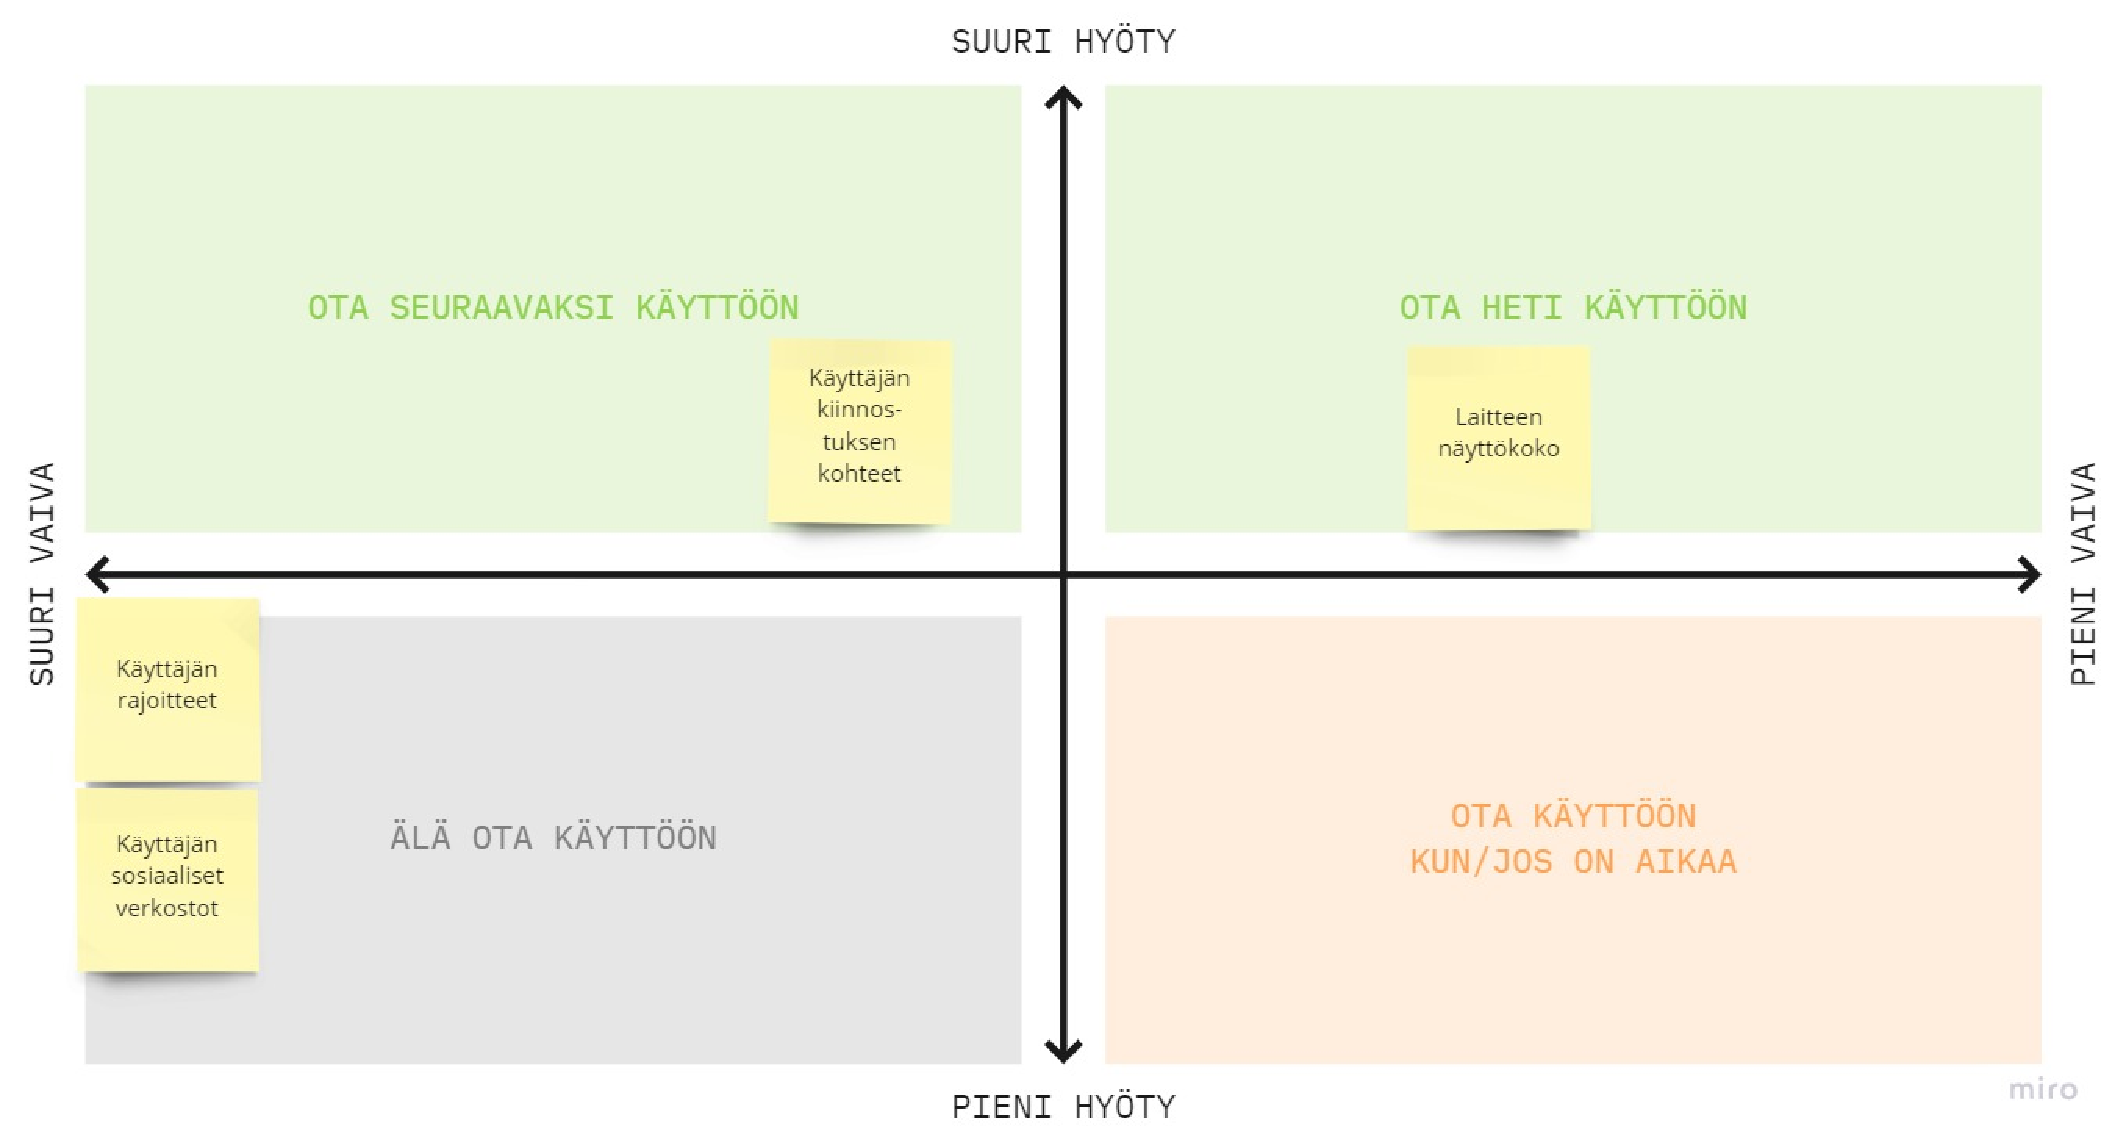
\includegraphics[width=\textwidth]{images/layout-priorization.pdf}
    \caption{Tärkeimmät sisällön asettelun personointimenetelmät.~\label{fig:layout-priorization}}
\end{figure}

\subsubsection{Valikoiden asettelu}

{\tiny\tabcolsep=3pt
    \begin{longtable}{p{2.5cm}|p{6cm}|p{0.5cm}p{0.5cm}p{0.5cm}|p{0.5cm}|p{0.5cm}p{0.5cm}p{0.5cm}|p{0.5cm}|}
        \multirow[t]{2}{*}{\textbf{Näkökulma}} & \multirow[t]{2}{*}{\textbf{Menetelmän kuvaus}} & \multicolumn{4}{c|}{\textbf{Vaivattomuus}} & \multicolumn{4}{c|}{\textbf{Hyöty}}                                                                                                                                                                                                                                                  \\\cline{3-10}
                                               &                                                & \vertical{\textbf{Toteutuksen helppous}}   & \vertical{\textbf{Monistettavuus}}  & \vertical{\textbf{Käyttö toimialalla}} & \vertical{\textbf{Yhteensä}} & \vertical{\textbf{Vaikutus käyttökokemukseen}~} & \vertical{\textbf{Kohdennuksen tarkkuus}} & \vertical{\textbf{Tulevaisuuden näkymät}} & \vertical{\textbf{Yhteensä}} \\
        \midrule
        \textbf{Käyttäjä}                                                                                                                                                                                                                                                                                                                                                                                                           \\
        \midrule
        Rajoitteet                                                                                                                                                                                                                                                                                                                                                                                                                  \\
        \midrule
        Ikä                                                                                                                                                                                                                                                                                                                                                                                                                         \\
        \midrule
        Sukupuoli                                                                                                                                                                                                                                                                                                                                                                                                                   \\
        \midrule
        Kulttuuritausta                                                                                                                                                                                                                                                                                                                                                                                                             \\
        \midrule
        Koulutustausta                                                                                                                                                                                                                                                                                                                                                                                                              \\
        \midrule
        Kiinnostuksen kohteet                                                                                                                                                                                                                                                                                                                                                                                                       \\
        \midrule
        Mieliala                                                                                                                                                                                                                                                                                                                                                                                                                    \\
        \midrule
        Sosiaaliset verkostot                                                                                                                                                                                                                                                                                                                                                                                                       \\
        \midrule
        \textbf{Käyttöympäristö}                                                                                                                                                                                                                                                                                                                                                                                                    \\
        \midrule
        Laitteen näyttökoko                                                                                                                                                                                                                                                                                                                                                                                                         \\
        \midrule
        Laitteen suorituskyky                                                                                                                                                                                                                                                                                                                                                                                                       \\
        \midrule
        Verkkoyhteyden laatu                                                                                                                                                                                                                                                                                                                                                                                                        \\
        \midrule
        Sijainti                                                                                                                                                                                                                                                                                                                                                                                                                    \\
        \midrule
        Aika                                                                                                                                                                                                                                                                                                                                                                                                                        \\
        \midrule
        Kirkkaus                                                                                                                                                                                                                                                                                                                                                                                                                    \\
        \midrule
        Äänekkyys                                                                                                                                                                                                                                                                                                                                                                                                                   \\
        \midrule
        Lämpötila ja sää                                                                                                                                                                                                                                                                                                                                                                                                            \\
        \midrule
        Liike                                                                                                                                                                                                                                                                                                                                                                                                                       \\
    \end{longtable}
}

\subsubsection{Typografia}

{\tiny\tabcolsep=3pt
    \begin{longtable}{p{2.5cm}|p{6cm}|p{0.5cm}p{0.5cm}p{0.5cm}|p{0.5cm}|p{0.5cm}p{0.5cm}p{0.5cm}|p{0.5cm}|}
        \multirow[t]{2}{*}{\textbf{Näkökulma}} & \multirow[t]{2}{*}{\textbf{Menetelmän kuvaus}} & \multicolumn{4}{c|}{\textbf{Vaivattomuus}} & \multicolumn{4}{c|}{\textbf{Hyöty}}                                                                                                                                                                                                                                                  \\\cline{3-10}
                                               &                                                & \vertical{\textbf{Toteutuksen helppous}}   & \vertical{\textbf{Monistettavuus}}  & \vertical{\textbf{Käyttö toimialalla}} & \vertical{\textbf{Yhteensä}} & \vertical{\textbf{Vaikutus käyttökokemukseen}~} & \vertical{\textbf{Kohdennuksen tarkkuus}} & \vertical{\textbf{Tulevaisuuden näkymät}} & \vertical{\textbf{Yhteensä}} \\
        \midrule
        \textbf{Käyttäjä}                                                                                                                                                                                                                                                                                                                                                                                                           \\
        \midrule
        Rajoitteet                                                                                                                                                                                                                                                                                                                                                                                                                  \\
        \midrule
        Ikä                                                                                                                                                                                                                                                                                                                                                                                                                         \\
        \midrule
        Sukupuoli                                                                                                                                                                                                                                                                                                                                                                                                                   \\
        \midrule
        Kulttuuritausta                                                                                                                                                                                                                                                                                                                                                                                                             \\
        \midrule
        Koulutustausta                                                                                                                                                                                                                                                                                                                                                                                                              \\
        \midrule
        Kiinnostuksen kohteet                                                                                                                                                                                                                                                                                                                                                                                                       \\
        \midrule
        Mieliala                                                                                                                                                                                                                                                                                                                                                                                                                    \\
        \midrule
        Sosiaaliset verkostot                                                                                                                                                                                                                                                                                                                                                                                                       \\
        \midrule
        \textbf{Käyttöympäristö}                                                                                                                                                                                                                                                                                                                                                                                                    \\
        \midrule
        Laitteen näyttökoko                                                                                                                                                                                                                                                                                                                                                                                                         \\
        \midrule
        Laitteen suorituskyky                                                                                                                                                                                                                                                                                                                                                                                                       \\
        \midrule
        Verkkoyhteyden laatu                                                                                                                                                                                                                                                                                                                                                                                                        \\
        \midrule
        Sijainti                                                                                                                                                                                                                                                                                                                                                                                                                    \\
        \midrule
        Aika                                                                                                                                                                                                                                                                                                                                                                                                                        \\
        \midrule
        Kirkkaus                                                                                                                                                                                                                                                                                                                                                                                                                    \\
        \midrule
        Äänekkyys                                                                                                                                                                                                                                                                                                                                                                                                                   \\
        \midrule
        Lämpötila ja sää                                                                                                                                                                                                                                                                                                                                                                                                            \\
        \midrule
        Liike                                                                                                                                                                                                                                                                                                                                                                                                                       \\
    \end{longtable}
}

\subsubsection{Värit}

{\tiny\tabcolsep=3pt
    \begin{longtable}{p{2.5cm}|p{6cm}|p{0.5cm}p{0.5cm}p{0.5cm}|p{0.5cm}|p{0.5cm}p{0.5cm}p{0.5cm}|p{0.5cm}|}
        \multirow[t]{2}{*}{\textbf{Näkökulma}} & \multirow[t]{2}{*}{\textbf{Menetelmän kuvaus}} & \multicolumn{4}{c|}{\textbf{Vaivattomuus}} & \multicolumn{4}{c|}{\textbf{Hyöty}}                                                                                                                                                                                                                                                  \\\cline{3-10}
                                               &                                                & \vertical{\textbf{Toteutuksen helppous}}   & \vertical{\textbf{Monistettavuus}}  & \vertical{\textbf{Käyttö toimialalla}} & \vertical{\textbf{Yhteensä}} & \vertical{\textbf{Vaikutus käyttökokemukseen}~} & \vertical{\textbf{Kohdennuksen tarkkuus}} & \vertical{\textbf{Tulevaisuuden näkymät}} & \vertical{\textbf{Yhteensä}} \\
        \midrule
        \textbf{Käyttäjä}                                                                                                                                                                                                                                                                                                                                                                                                           \\
        \midrule
        Rajoitteet                                                                                                                                                                                                                                                                                                                                                                                                                  \\
        \midrule
        Ikä                                                                                                                                                                                                                                                                                                                                                                                                                         \\
        \midrule
        Sukupuoli                                                                                                                                                                                                                                                                                                                                                                                                                   \\
        \midrule
        Kulttuuritausta                                                                                                                                                                                                                                                                                                                                                                                                             \\
        \midrule
        Koulutustausta                                                                                                                                                                                                                                                                                                                                                                                                              \\
        \midrule
        Kiinnostuksen kohteet                                                                                                                                                                                                                                                                                                                                                                                                       \\
        \midrule
        Mieliala                                                                                                                                                                                                                                                                                                                                                                                                                    \\
        \midrule
        Sosiaaliset verkostot                                                                                                                                                                                                                                                                                                                                                                                                       \\
        \midrule
        \textbf{Käyttöympäristö}                                                                                                                                                                                                                                                                                                                                                                                                    \\
        \midrule
        Laitteen näyttökoko                                                                                                                                                                                                                                                                                                                                                                                                         \\
        \midrule
        Laitteen suorituskyky                                                                                                                                                                                                                                                                                                                                                                                                       \\
        \midrule
        Verkkoyhteyden laatu                                                                                                                                                                                                                                                                                                                                                                                                        \\
        \midrule
        Sijainti                                                                                                                                                                                                                                                                                                                                                                                                                    \\
        \midrule
        Aika                                                                                                                                                                                                                                                                                                                                                                                                                        \\
        \midrule
        Kirkkaus                                                                                                                                                                                                                                                                                                                                                                                                                    \\
        \midrule
        Äänekkyys                                                                                                                                                                                                                                                                                                                                                                                                                   \\
        \midrule
        Lämpötila ja sää                                                                                                                                                                                                                                                                                                                                                                                                            \\
        \midrule
        Liike                                                                                                                                                                                                                                                                                                                                                                                                                       \\
    \end{longtable}
}

\subsubsection{Kuvien sovitus}

{\tiny\tabcolsep=3pt
    \begin{longtable}{p{2.5cm}|p{6cm}|p{0.5cm}p{0.5cm}p{0.5cm}|p{0.5cm}|p{0.5cm}p{0.5cm}p{0.5cm}|p{0.5cm}|}
        \multirow[t]{2}{*}{\textbf{Näkökulma}} & \multirow[t]{2}{*}{\textbf{Menetelmän kuvaus}} & \multicolumn{4}{c|}{\textbf{Vaivattomuus}} & \multicolumn{4}{c|}{\textbf{Hyöty}}                                                                                                                                                                                                                                                  \\\cline{3-10}
                                               &                                                & \vertical{\textbf{Toteutuksen helppous}}   & \vertical{\textbf{Monistettavuus}}  & \vertical{\textbf{Käyttö toimialalla}} & \vertical{\textbf{Yhteensä}} & \vertical{\textbf{Vaikutus käyttökokemukseen}~} & \vertical{\textbf{Kohdennuksen tarkkuus}} & \vertical{\textbf{Tulevaisuuden näkymät}} & \vertical{\textbf{Yhteensä}} \\
        \midrule
        \textbf{Käyttäjä}                                                                                                                                                                                                                                                                                                                                                                                                           \\
        \midrule
        Rajoitteet                                                                                                                                                                                                                                                                                                                                                                                                                  \\
        \midrule
        Ikä                                                                                                                                                                                                                                                                                                                                                                                                                         \\
        \midrule
        Sukupuoli                                                                                                                                                                                                                                                                                                                                                                                                                   \\
        \midrule
        Kulttuuritausta                                                                                                                                                                                                                                                                                                                                                                                                             \\
        \midrule
        Koulutustausta                                                                                                                                                                                                                                                                                                                                                                                                              \\
        \midrule
        Kiinnostuksen kohteet                                                                                                                                                                                                                                                                                                                                                                                                       \\
        \midrule
        Mieliala                                                                                                                                                                                                                                                                                                                                                                                                                    \\
        \midrule
        Sosiaaliset verkostot                                                                                                                                                                                                                                                                                                                                                                                                       \\
        \midrule
        \textbf{Käyttöympäristö}                                                                                                                                                                                                                                                                                                                                                                                                    \\
        \midrule
        Laitteen näyttökoko                                                                                                                                                                                                                                                                                                                                                                                                         \\
        \midrule
        Laitteen suorituskyky                                                                                                                                                                                                                                                                                                                                                                                                       \\
        \midrule
        Verkkoyhteyden laatu                                                                                                                                                                                                                                                                                                                                                                                                        \\
        \midrule
        Sijainti                                                                                                                                                                                                                                                                                                                                                                                                                    \\
        \midrule
        Aika                                                                                                                                                                                                                                                                                                                                                                                                                        \\
        \midrule
        Kirkkaus                                                                                                                                                                                                                                                                                                                                                                                                                    \\
        \midrule
        Äänekkyys                                                                                                                                                                                                                                                                                                                                                                                                                   \\
        \midrule
        Lämpötila ja sää                                                                                                                                                                                                                                                                                                                                                                                                            \\
        \midrule
        Liike                                                                                                                                                                                                                                                                                                                                                                                                                       \\
    \end{longtable}
}

\subsection{Yhteenveto}

Tähän yhteinen kuva kaikista menetelmistä.

\clearpage

\section{Yhteenveto}

\clearpage

\thesisbibliography{}
\printbibliography{}

\clearpage
\thesisappendix{}

\section{Esimerkki liitteestä\label{LiiteA}}

- Kuva tyypillisestä web-sivustosta jossa korostettu työn kannalta relevantit
osat, kuten rakenne, ilme, sisältö, saavutettavuus.

\end{document}
